\section{Related Work}
\begin{figure*}[t!]
  \centering
  \begin{subfigure}[t]{0.49\linewidth}
    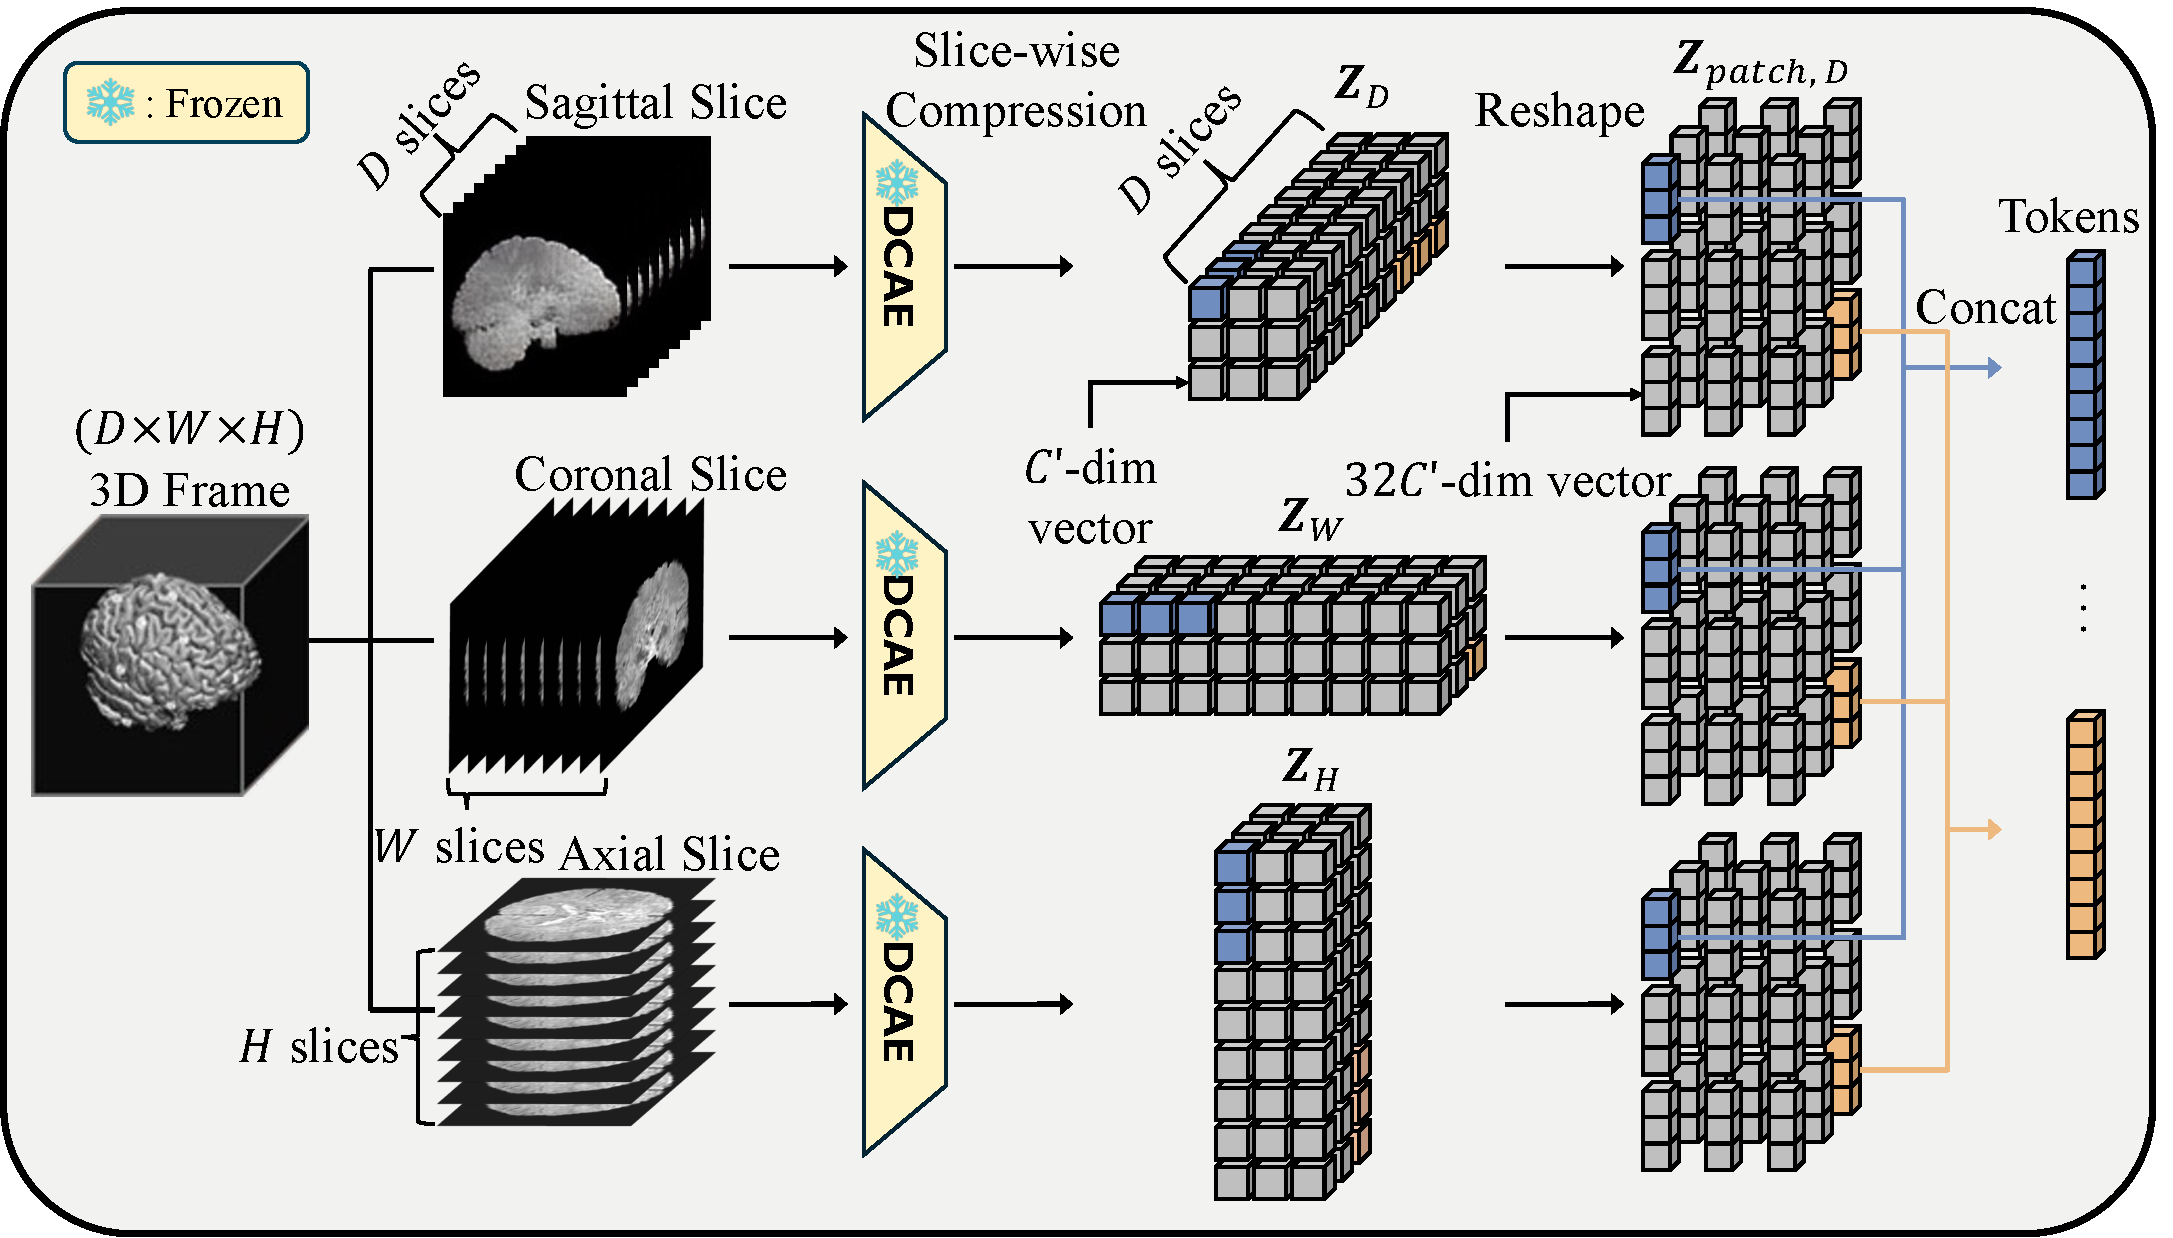
\includegraphics[width=\linewidth]{figures/a.pdf}
    \caption{Tokenization process of a 3D volume using a 2D encoder.}
  \end{subfigure}\hfill
  \begin{subfigure}[t]{0.49\linewidth}
    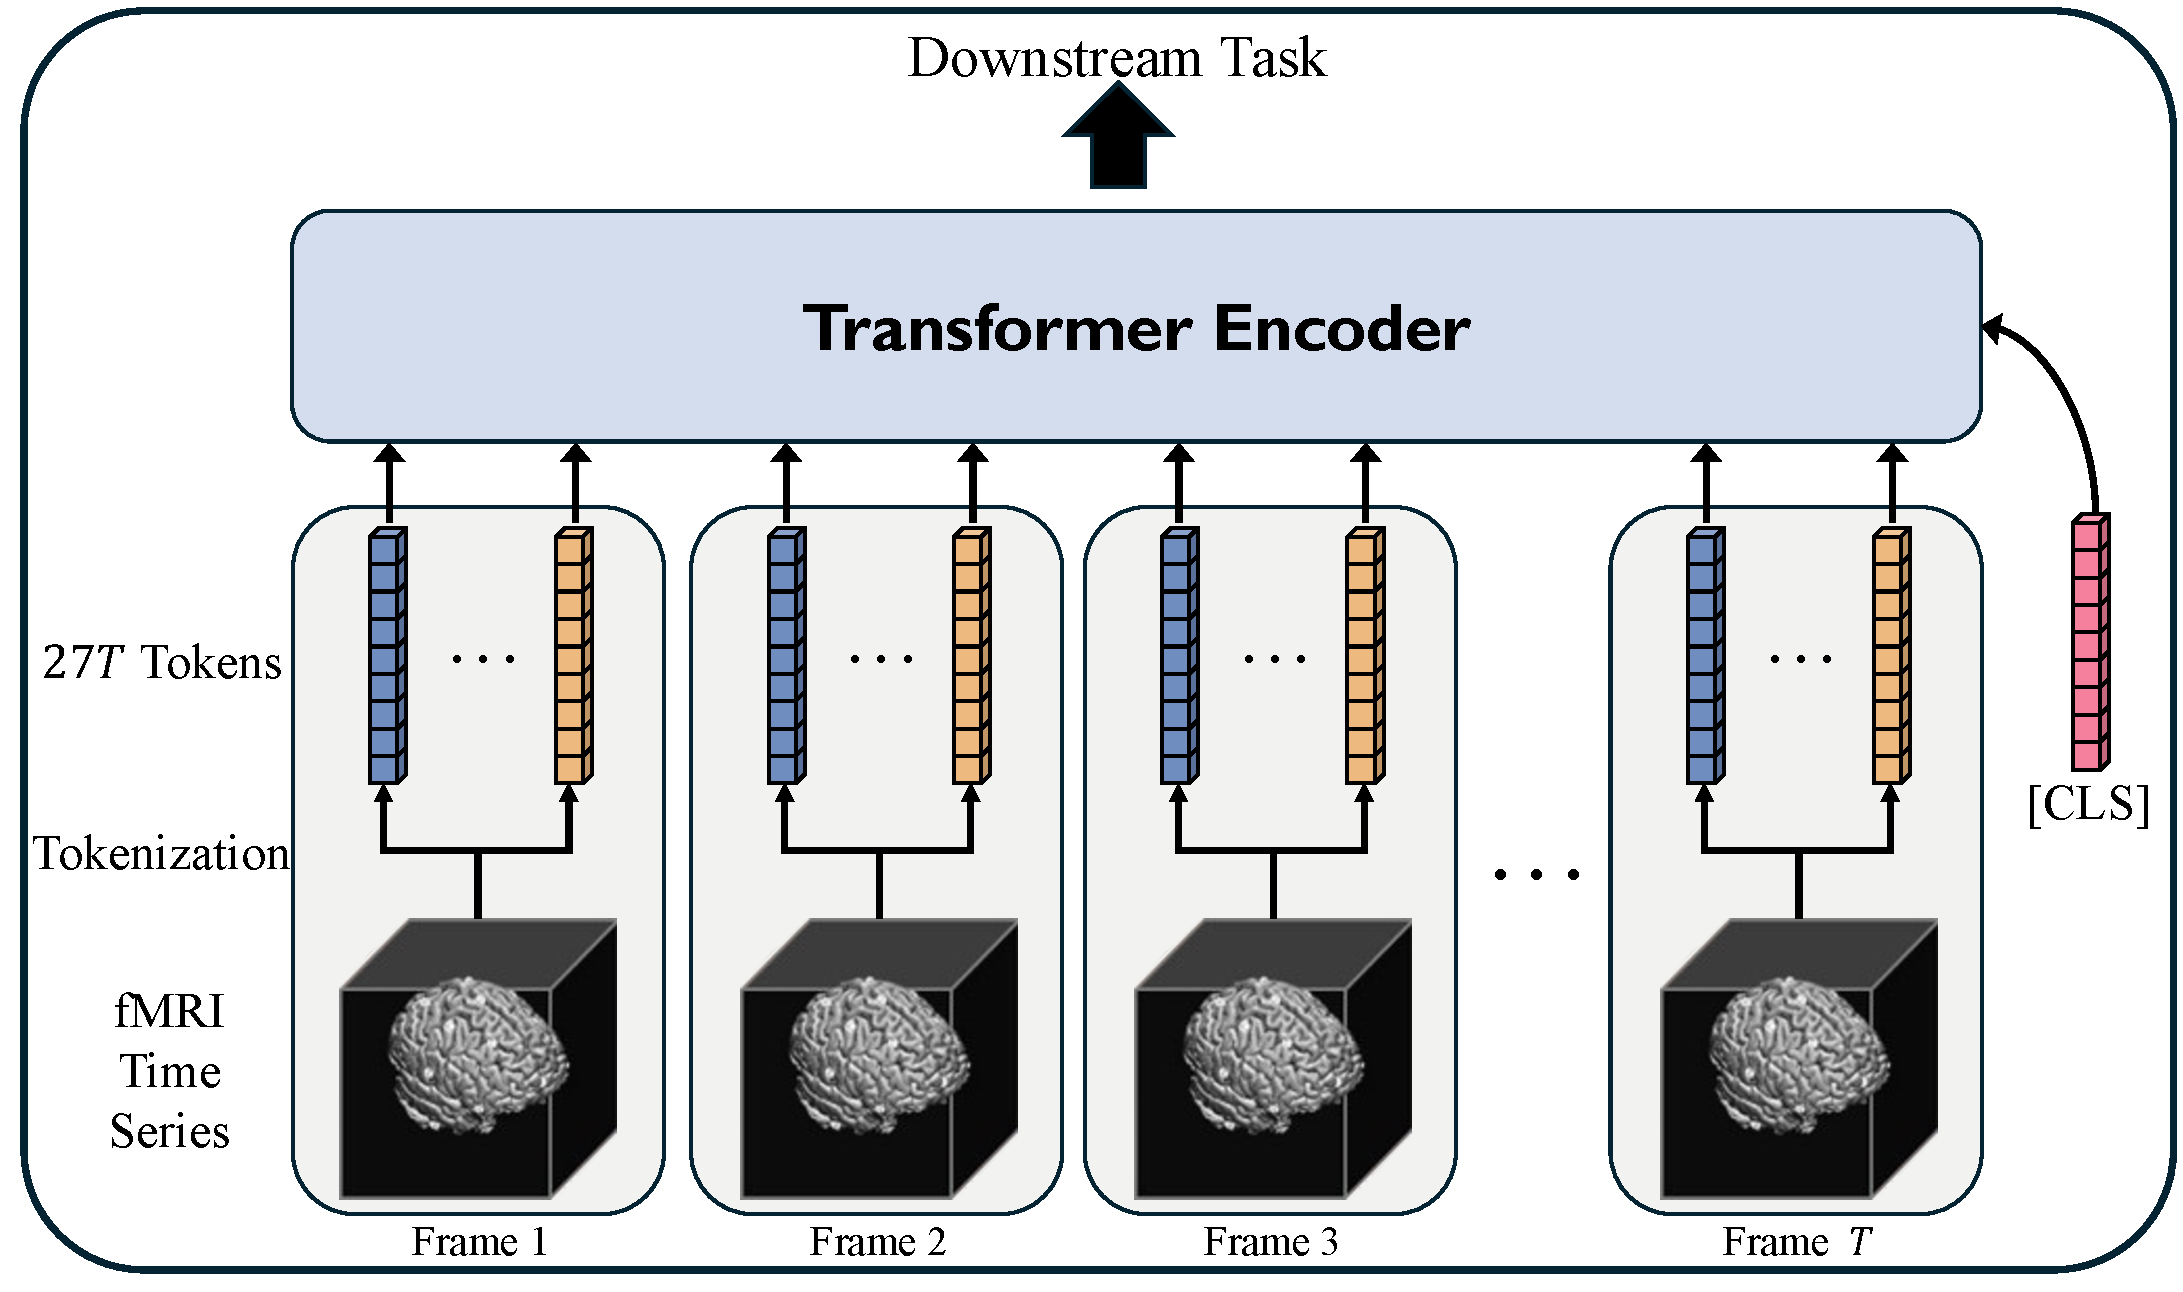
\includegraphics[width=\linewidth]{figures/b.pdf}
    \caption{Overview of {\ours}.}
  \end{subfigure}
  \caption{In {\ours}, each frame of the fMRI timeseries is tokenized by a 2D autoencoder, and the tokens are processed by a Transformer.}
  \label{fig:overview}
  \vspace{-3mm}
\end{figure*}
\label{sec:related_works}
\noindent \textbf{ROI-Based Methods.} ROI-based methods parcellate the brain into ROIs and average the BOLD signals within each. The signals are transformed into FC matrices by computing the correlation between the time series of the ROIs.
BrainNetCNN \citep{BNC} treats the FC matrix as a 2D image and uses edge-to-edge, edge-to-node, and node-to-graph convolutional filters to utilize topological locality in ROI-based networks. 
Brain Network Transformer \citep{BNT} adapts the Transformer architecture to process FC matrices as graphs of ROIs. 
meanMLP \citep{meanmlp} is a lightweight MLP-based model that applies the same MLP repeatedly across parcellated fMRI time-series and averages the resulting embeddings across time before a final classification layer. 
Brain-JEPA \citep{brainjepa} is a joint-embedding predictive architecture (JEPA) model pretrained on parcellated fMRI with spatiotemporal masking and gradient-based positioning. Even though computationally efficient, they are inherently limited by the strong pre-processing step that turns brain signals into FC matrices; it is heavily influenced by the choice of ROIs, and during the process, structural information as well as other signals can be discarded.

\noindent \textbf{Voxel-Based Methods.} Voxel-based methods process 4D fMRI volumes, enabling end-to-end learning of spatiotemporal features without ROI aggregation.
TFF \citep{TFF} operates on entire 4D volumes using a two-phase approach: self-supervised pretraining to reconstruct 3D volumes and fine-tuning. It captures fine-grained spatiotemporal dynamics, enabling transfer learning from unlabeled data.
SwiFT \citep{swift} extends the Swin Transformer to 4D fMRI volumes with a 4D window multi-head self-attention mechanism and absolute positional embeddings. 
Voxel-based methods are free from the issues with ROI-based models; however, they are burdened with a higher memory and computation load, as they need to deal with high-dimensional data.

\noindent \textbf{Self-Supervised Pretraining.}
Self-supervised learning (SSL) has emerged as a powerful pre-training framework for vision models, enabling scalable representation learning from unlabeled datasets.
MAE \citep{mae} introduces an asymmetric encoder-decoder architecture, where a high portion of input image patches are masked. Visible patches are encoded by Vision Transformer (ViT), and the decoder reconstructs the masked patches in pixel space. MAE demonstrated superior downstream task transfer, such as classification and segmentation.
SimMIM \citep{simmim} proposes a masked image modeling (MIM) framework using hierarchical transformers and a simple linear prediction head.
VideoMAE \citep{videomae} extends the MAE framework to videos by randomly applying masks on spatio-temporal cubes across spatio-temporal dimensions. The model reconstructs the masked cubes, learning dynamics, and long-range interactions.

\noindent \textbf{Deep Compression Autoencoder.}
Deep Compression Autoencoder (DCAE) \citep{DCAE} introduces an autoencoder framework for accelerating high-resolution diffusion models through extreme spatial compression ratios of up to 128$\times$. DCAE achieves superior reconstruction quality at high compression levels by residual autoencoding. Residual autoencoding utilizes non-parametric shortcuts that enable the model to learn residuals. The encoder downsample blocks adapt a space-to-channel operation, and the decoder upsample blocks use a channel-to-space operation. These non-parametric operations effectively preserve information without learned parameters.


